\documentclass[10pt]{beamer}
\usetheme{Madrid}
\usecolortheme{crane}
\usefonttheme{structurebold}




%\usecolortheme{seahorse}
\useinnertheme{rectangles}
\useoutertheme{infolines}
\usepackage{xcolor, natbib}
\usepackage[utf8]{inputenc}
\usepackage{tikz}
\usepackage{tabularx}
\usepackage{lipsum}
\usepackage{amsmath,graphicx,dsfont}
\usepackage{graphicx}
\usetikzlibrary{shapes,backgrounds,arrows,automata,snakes,shadows,positioning, mindmap}


\graphicspath{{figs/}}

%===================================
\newcommand{\Ccal}{\mathcal{C}}
\newcommand{\edgeunit}{1.5}
%\newcommand{\emph}[1]{\textcolor{Complement}{#1}}
\newcommand{\bleu}[1]{\textcolor{Cerulean}{#1}}
\newcommand{\pos}[1]{\textcolor{Darkgreen}{#1}}
\newcommand{\nega}[1]{\textcolor{Nicered}{#1}}
\newcommand\independent{\protect\mathpalette{\protect\independenT}{\perp}}\def\independenT#1#2{\mathrel{\rlap{$#1#2$}\mkern2mu{#1#2}}}
\newcommand{\Ncal}{\mathcal{N}}
\tikzset{%
    observed/.style={%
    scale=0.6,circle,draw=Framableulight,transform shape,fill=white,font=\Large}
}
\newcommand{\argmax}{\mathop{\mathrm{argmax}}}   
\newcommand{\backupbegin}{
   \newcounter{framenumberappendix}
   \setcounter{framenumberappendix}{\value{framenumber}}
}
\newcommand{\backupend}{
   \addtocounter{framenumberappendix}{-\value{framenumber}}
   \addtocounter{framenumber}{\value{framenumberappendix}} 
}

\makeatletter
\setbeamertemplate{footline}
{
  \leavevmode%
  \hbox{%
  \begin{beamercolorbox}[wd=.333333\paperwidth,ht=2.25ex,dp=1ex,center]{author in head/foot}%
    \usebeamerfont{author in head/foot}C. Ambroise %~~\beamer@ifempty{\insertshortinstitute}{}{(\insertshortinstitute)}
  \end{beamercolorbox}%
  \begin{beamercolorbox}[wd=.333333\paperwidth,ht=2.25ex,dp=1ex,center]{title in head/foot}%
    \usebeamerfont{title in head/foot} séminaire Agro Rennes
  \end{beamercolorbox}%
  \begin{beamercolorbox}[wd=.333333\paperwidth,ht=2.25ex,dp=1ex,right]{date in head/foot}%
    \usebeamerfont{date in head/foot}\insertshortdate{}\hspace*{2em}
    \insertframenumber{} / \inserttotalframenumber\hspace*{2ex} 
  \end{beamercolorbox}}%
  \vskip0pt%
}
\makeatother


\definecolor{Cerulean}{RGB}{16,61,75}
\definecolor{white}{RGB}{255,255,255}
\renewcommand{\textbf}[1]{\textcolor{Cerulean}{\bf#1}}
\setbeamercolor{structure}{bg=Cerulean}
\setbeamercolor{structure}{fg=white}
\setbeamercolor{frametitle}{bg=Cerulean}
\setbeamercolor{frametitle}{fg=white}
\setbeamercolor{title}{bg=Cerulean}
\setbeamercolor{title}{fg=white}
\setbeamercolor{block title}{fg=Cerulean}
\setbeamercolor{item}{fg=Cerulean}
\setbeamercolor{page number in head/foot}{fg=white, bg=Cerulean}
\setbeamercolor{author in head/foot}{fg=white, bg=Cerulean}
\setbeamercolor{institute in head/foot}{fg=white, bg=Cerulean}
\setbeamercolor{title in head/foot}{fg=white, bg=Cerulean}
\setbeamercolor{date in head/foot}{fg=white, bg=Cerulean}
\setbeamercolor{section in head/foot}{fg=white, bg=Cerulean}
\setbeamercolor{emph}{fg=red}


\renewcommand<>{\emph}[1]{%
  {\usebeamercolor[fg]{emph}\only#2 #1}%
}


% TikZ
\newcommand{\nodesize}{1em}
\tikzstyle{covariate}=[draw, minimum width=\nodesize, minimum height=\nodesize, inner sep=0, color=black]
\tikzstyle{covmiss}=[draw, minimum width=\nodesize, minimum height=\nodesize, inner sep=0, color=gray, text=gray]
\tikzstyle{observed}=[draw, circle, minimum width=\nodesize, inner sep=0, color=black]
\tikzstyle{edge}=[-, line width=1pt, color=black]
\tikzstyle{edgemiss}=[-, line width=1pt, dashed, color=gray]



%===================================
\definecolor{Framableu}{RGB}{12,91,122}
\definecolor{Framableulight}{RGB}{18,144,176}
\definecolor{Nicered}{RGB}{176,18,65}
%\definecolor{Nicered}{RGB}{141,14,52}
%\definecolor{Lightpink}{RGB}{229,177,218}
%\definecolor{Green}{RGB}{144,176,18}
%\definecolor{Lightcomplement}{RGB}{235,204,196}
%\definecolor{Darkgoldenrod}{RGB}{176,144,18}
%\definecolor{Darkomplement}{RGB}{122,43,12}
%\definecolor{Complement}{RGB}{176,50,18}
%\definecolor{Darkgreen}{RGB}{52,141,14}
%===================================
%\setbeamertemplate{itemize items}[square]
%\setbeamertemplate{blocks}[shadow=false]
%\setbeamertemplate{caption}{\raggedright\insertcaption\par}
%===================================
%\setbeamercolor{section in head/foot}{fg=white,bg=Framableu}
%\setbeamercolor{subsection in head/foot}{fg=white,bg=Framableulight}
%\setbeamercolor{author in head/foot}{bg=Framableu}
%\setbeamercolor{item}{fg=Framableulight}
%\setbeamercolor*{structure}{bg=Framableulight!20,fg=Framableulight}
%\setbeamercolor*{palette secondary}{use=structure,fg=white,bg=structure.fg!75}
%\setbeamercolor{section in toc}{fg=Framableu,bg=white}
%\setbeamercolor{frametitle}{fg=Framableu!80,bg=white}
%\setbeamercolor{block title}{fg=white, bg=Framableulight}  
%===================================





\title{Ecological network reconstruction from count data}

\author{Christophe Ambroise, Raphaëlle Momal,  Stéphane Robin}
\institute[]
{
  \inst{1}%
  UMR AgroParisTech / INRA MIA-Paris \\
  \inst{2}%
  LaMME, Evry
  }
\date{March$15^{\text{th}}$, 2019}


%#################################################################

\begin{document}

\begin{frame}
    \titlepage
\end{frame}

\section{Motivation}
%====================================================================
%====================================================================



\begin{frame}{Abundance Data}


\begin{block}{Jointly analysed species abundances in Ecology}
\begin{itemize}
	\item Metagenomics 
	\item Microbiology
	\item Ecology
\end{itemize}
\end{block}


\begin{block}{Understanding abundance data}
\begin{itemize}
\item  often analysed using species distribution model \citep{SDM}, 
where species are traditionally considered as disconnected entities. 
\item  biotic interactions are relevant descriptors of an ecosystem \citep{valiente,jordanoS}. 
\item  interactions can be conveniently represented by ecological networks
\end{itemize}
\end{block}

%\pause


\begin{itemize}
\item This work focuses on ecological network reconstruction based on observed species abundance data. 
\end{itemize}

\end{frame}



\begin{frame}{Interaction and statistics}

\begin{block}{Direct interactions (Causality ?)}
\begin{itemize}
\item  a useful network shall include only direct interactions between species. 
\item Indirect statistical association may be observed between two species either because they are both affected by the same environmental variations
\item any approach aiming at reconstructing ecological networks needs to account for covariates 
\end{itemize}
\end{block}


\end{frame}


%====================================================================
%====================================================================


%====================================================================
%====================================================================

\section{Network inference}
\subsection{General Framework}
%====================================================================
%===================================================================
%====================================================================



\begin{frame}{Graphical models: a statistical framework for network inference}
 \emph{Generic statistical model.}
  $$
  (Y_i)_{i = 1..n} \text{ iid } \sim P, 
   $$
   
   
 \begin{block}{Faithfulness.}
  
A distribution $P$  is said to be Markov faithful to a graph $G$ if, for
any triple (A, B, S) of disjoint subsets of nodes, it holds that



$$
\textrm{(S separates A from B in G)} \Leftrightarrow  A \independent B | S.
$$
\end{block}

\end{frame}


\begin{frame}{Graphical models: a statistical framework for network inference}
\emph{Example}:\bigskip
\begin{columns}
\begin{column}{0.3\linewidth}\hspace{0.5cm}
  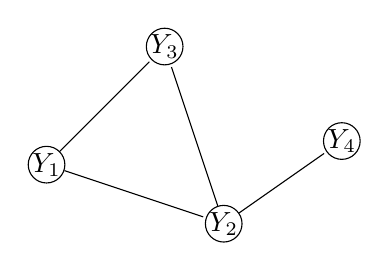
\begin{tikzpicture}	

      \tikzstyle{every edge}=[-,>=stealth',shorten >=1pt,auto,thin,draw]
		\node[observed] (Y1) at (0*\edgeunit, 0*\edgeunit) {$Y_1$};
		\node[observed] (Y2) at (1.5*\edgeunit, -0.5*\edgeunit) {$Y_2$};
		\node[observed] (Y3) at (1*\edgeunit, 1*\edgeunit) {$Y_3$};
		\node[observed] (Y4) at (2.5*\edgeunit, 0.2*\edgeunit) {$Y_4$};
		\path (Y1) edge [] (Y2)
        (Y1) edge [] (Y3)
        (Y2) edge [] (Y3)
        (Y2) edge [] (Y4);
	\end{tikzpicture}\\
\end{column}
\begin{column}{0.5\linewidth}
	\begin{itemize}
	\item Connected: all variables are dependant \bigskip
	\item Some are \emph{conditionally independent} (i.e. indirectly dependant)\\\bigskip
	 $Y_4$ is independent from $(Y_1, Y_3)$ conditionally on $Y_2$ \vspace{0.2cm}
\end{itemize}
\end{column}
\end{columns}
\pause
\begin{center}
    \[ P(Y_1, \dots, Y_p) \propto \prod_{C \in \Ccal_G} \psi_C(Y_C)  \propto  \psi_1(Y_1 ,Y_2, Y_3) \times \psi_2(Y_3, Y_4)\]
  where $\Ccal_G =$ set of maximal cliques of $G$.
\end{center}

\end{frame}
%====================================================================
%====================================================================

\frame{ \frametitle{Network inference}

  \emph{Network inference problem.}
  $$
  \text{Based on the dataset $Y = (Y_{ij})$, infer $G$.}
  $$

  \bigskip \bigskip \pause
  \emph{Critical issue.} There are $2^{p(p-1)/2}$ possible graphs
  $$
  \begin{array}{lcccc}
    p & 5 & 10 & 20 & 50 \\ \hline
    \text{\# graphs} & 10^3 & 10^{14} & 10^{57} & 10^{369}
  \end{array}
  $$
}


\begin{frame}{Practical influence of covariates}
%\begin{block}{What kind of statistical tools ?}
%\begin{itemize}
%\item Graphical Models:  formal probabilistic framework to describe the dependency structure between a set of variables. 
%\item Causality (intervention data)
%\end{itemize}
%\end{block}


\begin{figure}[H]
    \centering
    \begin{tabular}{ccccccc}
        \input{figs/FigGraphModel-Connected} & \qquad &
          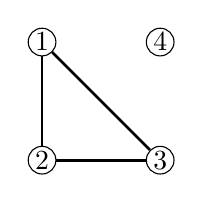
\begin{tikzpicture}
  \node[observed] (1) at (-0.5*\edgeunit,  .5*\edgeunit) {$1$};
  \node[observed] (2) at (-0.5*\edgeunit, -.5*\edgeunit) {$2$};
  \node[observed] (3) at ( 0.5*\edgeunit, -.5*\edgeunit) {$3$};
  \node[observed] (4) at ( 0.5*\edgeunit,  .5*\edgeunit) {$4$};
  \draw[edge] (1) to (2); \draw[edge] (2) to (3);  \draw[edge] (1) to (3); 
  \end{tikzpicture}
 & \qquad &
          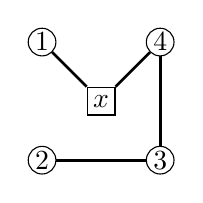
\begin{tikzpicture}
  \node[observed] (1) at (-0.5*\edgeunit,  .5*\edgeunit) {$1$};
  \node[observed] (2) at (-0.5*\edgeunit, -.5*\edgeunit) {$2$};
  \node[observed] (3) at ( 0.5*\edgeunit, -.5*\edgeunit) {$3$};
  \node[observed] (4) at ( 0.5*\edgeunit,  .5*\edgeunit) {$4$};
  \node[covariate] (x) at (0.0*\edgeunit,  .0*\edgeunit) {$x$};
  \draw[edge] (2) to (3); \draw[edge] (3) to (4); 
  \draw[edge] (x) to (1); \draw[edge] (x) to (4);
  \end{tikzpicture}
 & \qquad &
          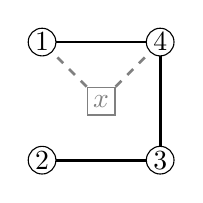
\begin{tikzpicture}
  \node[observed] (1) at (-0.5*\edgeunit,  .5*\edgeunit) {$1$};
  \node[observed] (2) at (-0.5*\edgeunit, -.5*\edgeunit) {$2$};
  \node[observed] (3) at ( 0.5*\edgeunit, -.5*\edgeunit) {$3$};
  \node[observed] (4) at ( 0.5*\edgeunit,  .5*\edgeunit) {$4$};
  \node[covmiss] (x) at (0.0*\edgeunit,  .0*\edgeunit) {$x$};
  \draw[edge] (2) to (3); \draw[edge] (3) to (4); 
  \draw[edgemiss] (x) to (1); \draw[edgemiss] (x) to (4);
  \draw[edge] (1) to (4); 
  \end{tikzpicture}
 \\
        ($a$) connected & & ($b$) disconnected & & ($c$) with covariate & & ($d$) missing covariate 
    \end{tabular}
    \caption{Examples of graphical models.}
    \label{fig:graphmodel}
\end{figure}

\end{frame}




\begin{frame}{Our problem}
\Large{\bleu{Data:}}\\ \normalsize{}
	\begin{itemize}
	\item \emph{Species}: bacteria, fungi...
	\item \emph{Abundances}: read counts from Next-Generation Sequencing technologies (metabarcoding) $\Rightarrow$ \bleu{$n\times p$ matrix $Y$}
	\item \emph{Covariates}: temperature, water depth...  $\Rightarrow$  \bleu{$n\times d$ matrix $X$}
	\item \emph{Offsets}: species-specific, sample-specific  $\Rightarrow$ \bleu{$n \times p$ matrix $O$}\bigskip
\end{itemize}
\Large{\bleu{Goal:}}\normalsize{}

	Infer the \emph{species interaction network} $\widehat{G}$ from count data $Y$, accounting for $X$ and $O$ : $$\widehat{G}=f(Y,X,O)$$

\end{frame}
%====================================================================
%====================================================================
\begin{frame}{Challenges}\large{
	\begin{itemize}
	\item  Statistical network inference \bigskip\bigskip
	\item Count data \bigskip\bigskip
	\item Offsets and covariates
\end{itemize}}
\end{frame}


\section{With count data}
\subsection{Model}

%====================================================================
%====================================================================

\begin{frame}{PLN model \only<3>{+ Graphical model}}
\begin{block}{Poisson log-Normal distribution \citep{AiH89}}
\[
            \left.
                \begin{array}{rl}
               \vspace{0.2cm}    Z_i \textit{ iid } &\sim \mathcal{N}_{d}(0,\Sigma\only<3>{\emph{_G}})\\
              \vspace{0.2cm}    &(Y_{ij})_j \independent |Z_i\\
                    Y_{ij}|Z_{ij} &\sim \mathcal{P}(e^{\only<2->{\emph{o_{ij}+x_i^{\text{T}}\Theta_j} +}Z_{ij}}) 
                   
                \end{array}
            \right \} Y \sim \mathcal{P\ell N}(\only<2->{\emph{O+X^{\text{T}}\Theta }}\only<1>{0}, \Sigma\only<3>{\emph{_G}})  
            \]
\end{block}

\begin{itemize}
    \item Dependency structure in the Gaussian latent layer
    \item Easy handling of multi-variate data 
  \only<2->{ \item Allow adjustment for covariates and offsets}
  \only<2->{\item Variational estimation algorithm \citep{CMR17}}
\end{itemize}
%\pause

\end{frame}


\begin{frame}
  \frametitle{Sparsity and Gaussian dependency}
  
  
   let $\mathbf{K} = (K_{ij})_{(i,j)\in\mathcal{P}^2} :=
      {\boldsymbol\Sigma}^{-1}$ be the \alert{concentration matrix}.
  \framesubtitle{General settings}
  
  
    \begin{block}{The graphical interpretation}<2->
    \vspace{-.2cm}
    \begin{equation*}
      Z_i \independent Z_j | Z_{\mathcal{P}\backslash \{i, j\}}  \Leftrightarrow K_{ij}=0  \Leftrightarrow \text{  edge }
      (i,j) \notin \text{ network},
    \end{equation*}
    since    $r_{ij|\mathcal{P}\backslash\{i,j\}}    =    -K_{ij}    /
    \sqrt{K_{ii} K_{jj}}$.
  \end{block}

  \vfill
  
  \onslide<2>{$\rightsquigarrow\mathbf{K}$  describes   the  graph  of
    \alert{conditional dependencies} of the hidden structure.}
\end{frame}


\begin{frame}{Gaussian graphical models}
  \framesubtitle{Example}

   
   $$ Z = \begin{pmatrix}
   Z_1 \\ 
   Z_2 \\ 
   Z_3
   \end{pmatrix}
   \text{, } \quad \quad \quad\Sigma = \begin{pmatrix}
   2 & 1 & -1 \\ 
   1 & 1.5 & -0.5 \\ 
   -1 & -0.5 & 1.5
   \end{pmatrix}$$
   
\vspace{1cm}
   $K = \Sigma^{-1} = \begin{pmatrix}
   1 & -0.5 & 0.5 \\ 
   -0.5 & 1 & 0 \\ 
   0.5 & 0 & 1
   \end{pmatrix}\text{, }\quad \quad \quad \mathcal{G}=$
   

   \vspace{-1.7cm} 
   \hspace{8cm}
    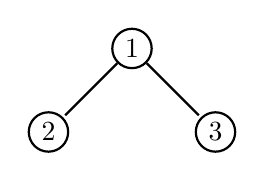
\begin{tikzpicture}[scale=0.5,->,>=stealth',shorten >=1pt,auto,node distance=1.5cm,
        thick,main node/.style={circle,draw,minimum size=0.5cm,inner sep=0pt]}]

    % Draw a 7,11 network
    % First we draw the vertices
    
%    \foreach \pos/\name in {{(1,2)/$1$}, {(0,1)/$2$}, {(1,1)/$3$},
%                            {(2,1)/$4$}, {(2,0)/$5$}}
%        \node[vertex] (\name) at \pos {$\name$};
%        
        
    \node[main node] (1) {$1$};
    \node[main node] (2) [below left of=1]  {$2$};
    \node[main node] (3) [below right of=1] {$3$};

       
       \path[-]
    (1) edge node {} (2)
        edge node {} (3);   

\end{tikzpicture}

   \vspace{1cm}
   \begin{itemize}
   
   \item Underlying graph $\mathcal{G} = (V,E)$, $V=\{1,\dots,p\}$
   \item The edge $\{i,j\}$ is in $ E $ if $K_{ij}\neq 0$\\
   \end{itemize}
   \begin{center}
   Inferring $\mathcal{G}$ $\Leftrightarrow $ inferring the support of $K$.

   \end{center}
   \end{frame}
 

   \begin{frame}{Inference of $K$ }
   \begin{block}{Estimate $K$ from data}
   \vspace{0.5cm}
   \begin{itemize}
   \item Maximum likelihood estimator:
   \end{itemize}
   \vspace{0.5cm}
   \begin{equation}
   \begin{aligned}
   & \hat{K}^{MLE} && = \underset{K}{\text{arg max }}\text{log det}(K) -\text{tr}(K\Sigma_n)\\
   & \quad && = \Sigma_n^{-1}
   \end{aligned}
   \end{equation}
   
   \vspace{0.5cm}
%   \begin{itemize}
%   \item Impossible to span all possible graphs: $2^{\frac{p(p-1)}{2}}$ of size $p$.
 %  \item Hypothesis on the structure of the support of $K$.
%   \end{itemize}
   \end{block}

    \begin{block}{Hypothesis on the structure of the support of $K$}
      \begin{itemize}
      \item Penalized Log-likelihood
      \item Tree hypothesis 
      \end{itemize}
    \end{block}

\end{frame}




\section{Tree averaging for network inference}

%====================================================================
\frame{ \frametitle{Tree-shaped network  on PLN latent layer }

\begin{center}
 \includegraphics[width=8cm]{spanningtrees.pdf}
\end{center}

 \begin{block}{PLN and spanning Tree}
\[
            \left.
                \begin{array}{rl}
                	 \vspace{0.2cm} 						T & \sim \prod_{kl} \emph{\beta_{kl}} /B\\ 
               \vspace{0.2cm}    Z_i | T \textit{ iid } &\sim \mathcal{N}_{d}(0,\emph{\Sigma_T})\\
              \vspace{0.2cm}    &(Y_{ij})_j \independent |Z_i| T\\
                    Y_{ij}|Z_{ij},T &\sim \mathcal{P}( e^{o_{ij}+x_i^{\text{T}}\Theta_j+Z_{ij}}) 
                   
                \end{array}
            \right \} Y \sim \mathcal{P\ell N}(O+X^{\text{T}}\Theta, \emph{\Sigma_T})  
            \]
\end{block}

}




\begin{frame}{Tree-shaped network  on PLN latent layer}


 \begin{block}{PLN and spanning Tree}
\[
            \left.
                \begin{array}{rl}
                	 \vspace{0.2cm} 						T & \sim \prod_{kl} \emph{\beta_{kl}} /B\\ 
               \vspace{0.2cm}    Z_i | T \textit{ iid } &\sim \mathcal{N}_{d}(0,\emph{\Sigma_T})\\
              \vspace{0.2cm}    &(Y_{ij})_j \independent |Z_i| T\\
                    Y_{ij}|Z_{ij},T &\sim \mathcal{P}( e^{o_{ij}+x_i^{\text{T}}\Theta_j+Z_{ij}}) 
                   
                \end{array}
            \right \} Y \sim \mathcal{P\ell N}(O+X^{\text{T}}\Theta, \emph{\Sigma_T})  
            \]
\end{block}


\begin{block}{Mixture of Trees}
$Z_i$ follows a mixture of centered Gaussian distributions with respective covariances matrices
$$Z_i \sim \sum_{T\in \mathcal{T}} P(T) \mathcal{N}(Z_i; 0,\Sigma_T)$$
\end{block}


\begin{itemize}
\item Both $Z$ and $T$ are latent variables
\end{itemize}

 \end{frame}


\subsection{Working with trees}
%====================================================================
%====================================================================

\begin{frame}{Why Spanning trees}

 \begin{description}

\item[Sparse structures: ]\begin{itemize}
\item[]
\end{itemize}
\emph{$\text{\#} \mathcal{G}_p = 2^{\frac{p(p-1)}{2}}$}  reduced to  \emph{$\text{\#} \mathcal{T}_p = p^{(p-2)}$}\bigskip\bigskip 

$$
  \begin{array}{lcccc}
    p & 5 & 10 & 20 & 50 \\ \hline
    \text{\# graphs} & 10^3 & 10^{14} & 10^{57} & 10^{369}\\
     \text{\# spanning trees} & 10^2 & 10^{8} & 10^{23} & 10^{81}
  \end{array}
$$


\pause
	\item[Suitable algebraic tool: ]\begin{itemize}
\item[]
\end{itemize}
Matrix tree theorem \citep{matrixtree}
$$\emph{ \sum_{T\in \mathcal{T}}}\prod_{(k,l) \in T} \psi_{k,l}(Y) = \det(L_{\psi(Y)})  \rightarrow \emph{\Theta (p^3)}$$

\end{description}
	
\center{
\textbf{Approach}: infer the network by \emph{averaging spanning trees}}
	
\end{frame}
%====================================================================
%====================================================================

\begin{frame}{Posterior probability for an edge}
  \emph{Prior on $T$:} factorizes over the edges:
  $$
  p(T) \propto \prod_{(j, k) \in T} \beta_{jk}
  $$


 The existence of an edge between variables $Z_j$ and $Z_k$ can be assessed by
  $$
  P((j, k) \in T \, | \, Z) \propto \sum_{T \ni (j, k)} p(T) p(Z\, | \,T)
  $$
  which depends on the prior $p(T)$.

\end{frame}


\begin{frame}{Tree averaging} 
\begin{center}
    

%\begin{tabular}{p{\linewidth}}
%\begin{tabularx}{\linewidth}{ccccl}
 \begin{tabular}{ccccl}
   \begin{tabular}{c}
	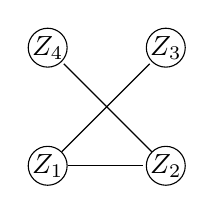
\begin{tikzpicture}
		
      \tikzstyle{every edge}=[-,>=stealth',shorten >=1pt,auto,thin,draw]
    
		\node[observed] (Z1) at (0*\edgeunit, 0*\edgeunit) {$Z_1$};
		\node[observed] (Z2) at (1*\edgeunit, 0*\edgeunit) {$Z_2$};
		\node[observed] (Z3) at (1*\edgeunit, 1*\edgeunit) {$Z_3$};
		\node[observed] (Z4) at (0*\edgeunit, 1*\edgeunit) {$Z_4$};
		\path (Z1) edge [] (Z2)
        (Z1) edge [] (Z3)
        (Z2) edge [] (Z4);
   
	\end{tikzpicture}\\
	\footnotesize{$P\{T = T_1 | Z\}$}
	   \end{tabular}
	   & 
	   \hspace{-.05\textwidth}% \pause
	   \begin{tabular}{c}
		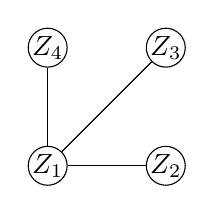
\begin{tikzpicture}
		\tikzstyle{every observed}=[draw=none,text=black,scale=0.5,
      transform shape,circular drop shadow] 
		\node[observed] (Z1) at (0*\edgeunit, 0*\edgeunit) {$Z_1$};
		\node[observed] (Z2) at (1*\edgeunit, 0*\edgeunit) {$Z_2$};
		\node[observed] (Z3) at (1*\edgeunit, 1*\edgeunit) {$Z_3$};
		\node[observed] (Z4) at (0*\edgeunit, 1*\edgeunit) {$Z_4$};
		
		\path (Z1) edge [] (Z2)
        (Z1) edge [] (Z3)
        (Z1) edge [] (Z4);
		\end{tikzpicture} \\
		\footnotesize{$P\{T = T_2 | Z\}$}
	   \end{tabular}
	   &
	   \hspace{-.05\textwidth} %\pause
	   \begin{tabular}{c}
		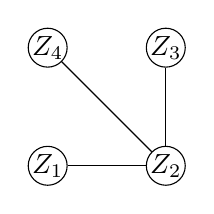
\begin{tikzpicture}
		\tikzstyle{every observed}=[draw=none,text=black,scale=0.5,
      transform shape,circular drop shadow] 
		\node[observed] (Z1) at (0*\edgeunit, 0*\edgeunit) {$Z_1$};
		\node[observed] (Z2) at (1*\edgeunit, 0*\edgeunit) {$Z_2$};
		\node[observed] (Z3) at (1*\edgeunit, 1*\edgeunit) {$Z_3$};
		\node[observed] (Z4) at (0*\edgeunit, 1*\edgeunit) {$Z_4$};
		
		\path (Z1) edge [] (Z2)
        (Z2) edge [] (Z3)
        (Z2) edge [] (Z4); 
		\end{tikzpicture}\\
		\footnotesize{$P\{T = T_3 | Z\}$}
	   \end{tabular}
	   &
	   \hspace{-.05\textwidth}% \pause
	   \begin{tabular}{c}
		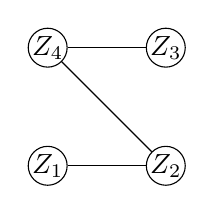
\begin{tikzpicture}
		\tikzstyle{every observed}=[draw=none,text=black,scale=0.5,
      transform shape,circular drop shadow] 
		\node[observed] (Z1) at (0*\edgeunit, 0*\edgeunit) {$Z_1$};
		\node[observed] (Z2) at (1*\edgeunit, 0*\edgeunit) {$Z_2$};
		\node[observed] (Z3) at (1*\edgeunit, 1*\edgeunit) {$Z_3$};
		\node[observed] (Z4) at (0*\edgeunit, 1*\edgeunit) {$Z_4$};
		 
		\path (Z1) edge [] (Z2)
        (Z3) edge [] (Z4)
        (Z2) edge [] (Z4);
		\end{tikzpicture} \\
		\footnotesize{$P\{T = T_4 | Z\}$}
	   \end{tabular}
	   & \hspace{-.06\textwidth} 
	   \huge{\emph{...}}\normalsize   \\ \\
	   \\% \pause
	   \begin{tabular}{l}
		Compute edge\\
		probabilities:
	   \end{tabular}
	   &
	   \hspace{-.05\textwidth}
	   \begin{tabular}{c}
		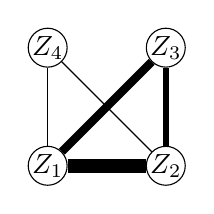
\begin{tikzpicture}
		\node[observed] (Z1) at (0*\edgeunit, 0*\edgeunit) {$Z_1$};
		\node[observed] (Z2) at (1*\edgeunit, 0*\edgeunit) {$Z_2$};
		\node[observed] (Z3) at (1*\edgeunit, 1*\edgeunit) {$Z_3$};
		\node[observed] (Z4) at (0*\edgeunit, 1*\edgeunit) {$Z_4$};
		\draw [line width=5pt] (Z1) -- (Z2); 
		\draw [line width=3pt] (Z1) -- (Z3); 
		\draw [line width=.5pt] (Z1) -- (Z4); 
		\draw [line width=2pt] (Z2) -- (Z3); 
		\draw [line width=.5pt] (Z2) -- (Z4); 
 %		\draw [line width=.5pt] (Z3) -- (Z4); 
		\end{tikzpicture}\\
		\emph{$P\{(j, k) \in T | Z\}$}
	   \end{tabular}
	   &
	  \hspace{-.05\textwidth} %\pause
	   \begin{tabular}{l}
		Thresholding\\
		probabilities:
	   \end{tabular}
	   &
	   \hspace{-.05\textwidth}
	   \begin{tabular}{c}
		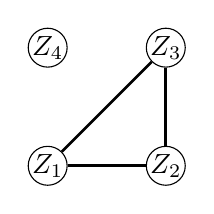
\begin{tikzpicture}
		\node[observed] (Z1) at (0*\edgeunit, 0*\edgeunit) {$Z_1$};
		\node[observed] (Z2) at (1*\edgeunit, 0*\edgeunit) {$Z_2$};
		\node[observed] (Z3) at (1*\edgeunit, 1*\edgeunit) {$Z_3$};
		\node[observed] (Z4) at (0*\edgeunit, 1*\edgeunit) {$Z_4$};
		\draw [line width=1pt] (Z1) -- (Z2); 
		\draw [line width=1pt] (Z1) -- (Z3); 
% 		\draw [line width=1pt] (Z1) -- (Z4); 
		\draw [line width=1pt] (Z2) -- (Z3); 
% 		\draw [line width=.1pt] (Z2) -- (Z4); 
% 		\draw [line width=1pt] (Z3) -- (Z4); 
		\end{tikzpicture}\\
		\emph{$P\{(j, k) \in T | Z\}$}
	   \end{tabular}
	   &
	 \end{tabular}
   % \end{tabular}
   %\end{tabularx}
   \end{center}
\end{frame}
%====================================================================
%====================================================================


\begin{frame}{Tree structured data}
\begin{columns}
 \begin{column}{0.7\linewidth}
 \begin{itemize}
    \item Data dependency structure relies on a tree \vspace{1cm}
    \item Likelihood \emph{factorizes on nodes and edges} \citep{ChowLiu}:
    \end{itemize}
 \end{column}
 \begin{column}{0.3\linewidth}
 \begin{center}
     \includegraphics[width=3cm]{arbredependance.PNG}   
    \end{center}
 \end{column}
\end{columns}

\[\mathds{P}(Z|T) =\prod_{j=1}^d \mathds{P}(Z_j)\prod_{k,l \in T}\psi_{kl}(Z) \hspace{0.3cm},\]

Where \[ \psi_{kl}(Z) = \frac{\mathds{P}(Z_k,Z_l)}{\mathds{P}(Z_k)\times \mathds{P}(Z_l)}.\]\\
\vspace{0.4cm}
\textbf{Rmq} : with standardised gaussian data, $\hat{\Psi} = [\hat{\psi_{kl}}] \propto (1-\hat{\rho_Z}^2)^{-1/2}$
\end{frame}
%====================================================================
%====================================================================

\begin{frame}{Direct EM algorithm ?}
\footnotesize 
\begin{itemize}
    \item \bleu{Complete likelihood :}

 \[ \mathds{P}(Y,Z,T) = \color{olive}\mathds{P}(T)\color{black}\times\color{blue}\mathds{P}(Z|T)\color{black}\times\color{orange}\mathds{P}(Y|Z)\]
 
\begin{align*}
 \log(\mathds{P}(Y,Z,T)) &= \sum_{k,l} \mathds{1}_{\{(k,l) \in T\}} (\color{olive}\log(\beta_{kl})\color{black} + \color{blue}\log(\psi_{kl}(Z)) \color{black})-\color{olive}\log(B)\color{black} \\
 &+\sum_k (\color{blue} \log(\mathds{P}(Z_k))\color{black} + \color{orange}\log(\mathds{P}(Y_k|Z_k))\color{black})
 \end{align*}
 
 \pause
 \item \bleu{Conditional expectation :}
\end{itemize}
\begin{align*}
    \mathds{E}_\theta[\log(\mathds{P}(Y,Z,T))|Y] =&\sum_{k,l\in V} \mathds{P}((k,l) \in T|Y) \log(\beta_{kl}) + \mathds{E}[\mathds{1}_{\{(k,l) \in T\}}\emph{\log(\psi_{kl}(Z)|Y)}]\\
& +\sum_k \emph{\mathds{E}[\log(\mathds{P}(Z_k)) | Y]} + \mathds{E}[\log(\mathds{P}(Y_k|Z_k)) | Y]-\log(B)
\end{align*} 

\normalsize 
\end{frame}
%====================================================================
%====================================================================


\begin{frame}{Two steps solution}
   The \emph{{\fontfamily{qcr}\selectfont
PLNmodels}} package approximates the distribution parameters:
    \vspace{0.3cm}
    \begin{enumerate}
        \item Approximate $\hat{\Sigma}_Z$ \vspace{0.2cm}
        \item Apply EM mixture tree to $Z \sim \mathcal{N}(0,\hat{\Sigma}_Z)$\\
    \end{enumerate}
\vspace{1.5cm}
Simplified conditional expectation writing:\\
\vspace{0.2cm}\small
\[\mathds{E}_\theta[\log(\mathds{P}(Z,T))|Z] =\sum_{k,l}  \emph{\mathds{P}((k,l) \in T|Z)}\times\log(\beta_{kl}\psi_{kl})-\log(B) +\sum_k \log(\mathds{P}(Z_k))\]
\normalsize 
\center{$\Rightarrow$  \textbf{EM algorithm }\footnotesize  (E: \citet{kirshner}, M: \citet{MeilaJaak}) }\vspace{0.2cm} \normalsize
\end{frame}

\begin{frame}{EMtree algorithm}
\begin{description}
\item [Input: ] \hspace{0.35cm}Abundance data, covariates, offsets\vspace{0.2cm}

\item [1rst step: ] \hspace{0.3cm}VEM algorithm to \emph{fit PLN model} $\Rightarrow$  $\hat{\theta}$, $\hat{\Sigma}_Z$. \vspace{0.2cm}
\item [2nd step: ] \hspace{0.3cm}EM algorithm to \emph{update the $\beta_{jk}$} $\Rightarrow$ conditional probabilities for all edges.\\ \hspace{0.3cm} 
\pause \bigskip
\item [Thresholding: ] Select edges with probability above the probability of edges in a tree drawn uniformly (\emph{$2/p$})\vspace{0.2cm}
\item [Resampling: ] \hspace{0.25cm}Strengthen the results: only edges selected in more than \emph{$80\%$} of $S$ sub-samples are kept.
\end{description} \bigskip

Available for download at \url{https://github.com/Rmomal/EMtree}
\begin{figure}
    \centering
    \includegraphics[width=0.6cm]{github.png}
\end{figure}
\end{frame}

\section{Evaluating performances}

\subsection{}
%====================================================================
%====================================================================

\begin{frame}{Evaluation strategy}

%%---------------


%%---------------


\emph{Alternatives:}\\
 Two methods  on \bleu{transformed counts, no covariates}:\\
    \begin{itemize}
        \item \emph{SpiecEasi} algorithm \citet{kurtz} : centered log-ratio (clr) transformation
        \item \emph{gCoda} \citet{gcoda} : log transformation to the relative counts
    \end{itemize}
    
   \begin{block}{Principles} 
  Both methods assume that 
 \begin{itemize}
 \item the transformed counts have a Gaussian distribution, 
\item that ecological networks are sparse.
 \item The network is then reconstructed using the graphical lasso \citep{GLasso}.
 \end{itemize}
 \end{block}
    
    
  One taking \emph{raw counts and covariates}:\\
    \begin{itemize}
        \item \emph{MInt} \citet{MInt} (uses PLN model): same PLN model (without Trees) and Graphical Lasso
    \end{itemize}
    
\end{frame}

\begin{frame}‘{Simulation design}
\begin{enumerate}
     \item Choose  \emph{$G$} and define  \emph{$\Sigma_G$} accordingly
     \item Sample count data \emph{$Y$} from $\mathcal{P\ell N}(X,\Sigma_G)$ 
     \item Infer the network with \emph{EMtree},  \emph{SpiecEasi},  \emph{gCoda}, and  \emph{MInt} 
     \item Compare results with  presence/absence of edges (\emph{FDR}, \emph{AUC})
\end{enumerate}


\end{frame}

\begin{frame}{Simulation settings}

\begin{block}{Difficulty}
\begin{itemize}
 \item  easy setting ($n=100$, $p=20$) 
 \item hard setting ($n=50$, $p=30$).
\end{itemize}
\end{block}

\begin{block}{Network Structure}
\begin{itemize}
\item  Erd\"os
\item  Cluster
\item  Scale free
\end{itemize}
\end{block}

\end{frame}

%====================================================================
%====================================================================

\subsection{Results}
\begin{frame}{Difficulty level}
\begin{figure}
    \centering
       \includegraphics[width=8.5cm]{panel_TPFN.png} 
\end{figure}

\end{frame}
\begin{frame}{Network density}
    
 \begin{figure}[H]
  \centering
   \includegraphics[width=\linewidth]{panel_npFav.png}\\
  \includegraphics[width=\linewidth]{panel_dense.png}
  \caption{\tiny{Effect of Erdös and Cluster structures on the evolutions of AUC median and inter-quartile intervals for parameters $n$, $p$ and $ratio$. \textit{Top}: densities set to $2/p$, \textit{bottom}: densities set to $5/p$.}}
  \label{panelErdClust}
\end{figure}

\end{frame}


\begin{frame}{Running Times}
\begin{table}[H]
\centering
\begin{tabular}{l | rr | rr}
& $n < 50$& $n\geq 50$  & $p < 20$& $p\geq 20$ \\  \hline
  EMtree    &   0.41 (0.11)	&   0.6  (0.15) &   0.38 (0.12) &    0.71 (0.21)      \\ 
  gCoda     &   0.12 (0.47)	&   0.07 (0.03) &   0.05 (0.03) &    0.09 (0.06)     \\ 
  SpiecEasi &   2.41 (0.25)	&   2.41 (0.25) &   2.39 (0.25) &    2.42 (0.25)      \\ 
   \hline
\end{tabular}
\caption{Median and standard-deviation of running times for each method in seconds, for $n$ and $p$ parameters. corresponding to Erdös and cluster structures with $5/p$ densities.}
\label{timeDenser}
\end{table}



\end{frame}
%====================================================================
%====================================================================


\section{Application}
\subsection{Oak data}

%====================================================================
%====================================================================

\begin{frame}{Oak Mildew}
\begin{columns}
\begin{column}{5cm}
\begin{figure}[htp]
\centering
\includegraphics[scale=0.07]{EA.jpg}
\caption{\textit{Pathogen Erysiphe alphitoides (EA).}}
\end{figure}
\end{column}
\begin{column}{6cm}
\begin{figure}[htp]
\centering
\includegraphics[scale=0.1]{mildew.jpg}
\caption{Oak leaf with powdery mildew.}
\end{figure}
\end{column}
\end{columns}
\vspace{0.5cm}
Metabarcoding of oak tree leaves microbiome \citep{jakuch}.\\

\begin{itemize}
	\item 114 sample of 94 bacterial/fungal-OTUs (Operational Taxonomic Unit)
	\item Different read depth for bacteria and fungi
	\item covariates: tree status; distance to ground, to trunk and to base of the branch.
\end{itemize}
\end{frame}
%====================================================================
%====================================================================

\begin{frame}{Inferred networks}

 
    \begin{figure}[htp]
\centering
\includegraphics[width=12cm]{oak_nets.png}
\end{figure}


\begin{itemize}
\item 10 neighbours for the pathogen Ea and 11 key-player OTUs. 
\item accounting for the covariates affects the network density, and the list of key-players.
\item  In addition, the connections of the pathogen Ea are greatly modified, highlighting changes in the microbiome of infected trees due to this agent.
\item  EMtree identifies three potential neighbors to the Ea  and two key-players in these networks, which were not identified by \citet{jakuch}. 
 \end{itemize}


\end{frame}

\begin{frame}{Selection Threshold}
\begin{figure}[H]
    \centering
    \includegraphics[width=8cm]{QET_Barans.png}
    \caption{Evolution of the quantity of selected edges along with the selection threshold on Fatala fish data.}
\end{figure}

\end{frame}


%-----------------------------
%---------------------------
\begin{frame}{Conclusion}
\begin{description}
\item[Contributions:] 
\begin{itemize}
\item[]  
	\item Formal probabilistic model for network inference with \emph{count data}
	\item Inclusion of \emph{offsets} and \emph{covariates}
	\item  Variational estimation algorithm
\end{itemize}
\bigskip 
\item[Perspectives:]

\begin{itemize}
\item[]  
	\item Taking spatial position into account
	\item Improving precision of computation
	\item Network comparison
	\item Missing major actor (species/covariates)	
	\item Model for the inference in the observed counts layer
\end{itemize}
\end{description}
\end{frame}
%====================================================================
%====================================================================


\begin{frame}{Acknowledgments}

Special thanks :\\
\begin{description}
\item[PLN team] Julien Chiquet (MIA-Paris), Mahendra Mariadassou (INRA Jouy)
\item[Data] Corinne Vacher (INRA Bordeaux)
\end{description}

\begin{center}
	\includegraphics[width=0.25\linewidth]{logo_inra.jpg}\hspace{0.1cm}
	\includegraphics[width=0.25\linewidth]{agro.PNG}
	\includegraphics[width=0.25\linewidth]{lmh.png}\hspace{0.1cm}
	\includegraphics[width=0.15\linewidth]{upsud.jpg}
    
\end{center}

\end{frame}
\appendix
\backupbegin

\begin{frame}{Conditional probability computation}
\footnotesize
\begin{exampleblock}{Kirchhoff's theorem (matrix tree, \cite{AiH89})}
For all $W=(a_{kl})_{k,l}$ a symmetric matrix, the corresponding Laplacian $Q(W)$ is defined as follows:
 \[\mathcal{Q}_{uv}(W)=
 \begin{cases}
     -a_{uv} & 1\leq u<v \leq n\\
    \sum_{i=1}^n a_{vi} & 1\leq u=v \leq n.
\end{cases}
\]
Then for all $u$ et $v$:
    \[ |Q^*_{uv}(W)|=\sum_{T\in\mathcal{T}} \prod_{\{k,l\}\in E_T} a_{kl} \]
\end{exampleblock}
\begin{align*}
  \mathds{P}((k,l)\in T | Z)&=\sum_{T\in \mathcal{T} : (k,l)\in T}\mathds{P}( T | Z) = \frac{\sum_{(k,l)\in T} \mathds{P}(T)\mathds{P}(Z|T)}{\sum_{T} \mathds{P}(T)\mathds{P}(Z|T)}\\
 &=\emph{1- \frac{|Q^*_{uv}(\beta\Psi^{-kl})|}{|Q^*_{uv}(\beta\Psi)|}}\\
 &= \tau_{kl}
 \end{align*}
 
\end{frame}



%====================================================================
%====================================================================

\subsection{M step}
\normalsize 
\begin{frame}{M step}
\textbf{Goal} : optimization of weights $\beta_{kl}$.\\
\vspace{1cm}
\[\argmax_{\beta_{kl}} \left\{\sum_{k,l\in V} \tau_{kl}(\emph{\log(\beta_{kl})} + \log(\psi_{kl}) ) -\emph{\log(B)} +\sum_k \log(\mathds{P}(Z_k))\right\}\]

  \vspace{1cm}
  
 \[\text{With high combinatorial complexity of } B = \sum_{T\in\mathcal{T}} \prod_{k,l\in T} \beta_{kl}\]
 
 \begin{center}
     How to compute \Large{$\frac{\partial B}{\partial\beta_{kl}}$ }?
 \end{center}
\end{frame}
 %====================================================================
%====================================================================

 \begin{frame}{$\beta_{kl}$ update}
 \footnotesize 
 \begin{exampleblock}{A result from Meil{\u{a}} \cite{MixtTrees}}
Inverting a minor of the laplacien $Q$, we define M : 
\[\begin{cases}
    M_{uv} = [\mathcal{Q}^{*-1}]_{uu} + [\mathcal{Q}^{*-1}]_{vv} -2[\mathcal{Q}^{*-1}]_{uv} & u,v < n\\
    M_{nv} =M_{vn} =[\mathcal{Q}^{*-1}]_{vv} & v<n\\
     M_{vv} =0.
   \end{cases}\]
On peut montrer que :
\[ \frac{\partial|Q^*_{uv}(W)|}{\partial \beta_{kl}} = M_{kl} \times |Q^*_{uv}(W)|\]
\end{exampleblock}
\[ \frac{\partial\mathds{E}_\theta[\log(\mathds{P}(Z,T))|Z]}{\partial\beta_{kl}} =\frac{ \tau_{kl} }{\beta_{kl}} - \frac{1}{B}
\frac{\partial B}{\partial\beta_{kl}}
\]


\emph{
   \large{\[\hat{\beta}_{kl}^{h+1} = \frac{\tau_{kl}^h}{M_{kl}^h}\]}
}
 \end{frame}

\begin{frame}[allowframebreaks]
\bibliographystyle{apalike}
{\tiny
    \bibliography{biblio3.bib}}
\frametitle{References}
%\bibliography{cellcite}
\end{frame}\backupend
%====================================================================
%====================================================================

\end{document}